% !TEX root = ../main.tex

\chapter{Introduction}

Decentralized Finance (DeFi) refers to a blockchain-based financial system that operates without intermediaries like banks, where transactions are correctly (under reasonable security assumptions) executed by a peer-to-peer network of validators. In blockchains like Ethereum, anyone can participate in the system at any time as either a user and/or a validator without any registration or permission. For this reason, blockchains are commonly described as permissionless. Thus DeFi is permissionless finance where anyone can offer new services or use the services that have been offered. This does not mean it is legal to use in all cases and jurisdictions, however, without validation of identities or citizenships, any laws or regulations can generally be circumvented without much technical effort.

As one might imagine, an arena of permissionless financial services is likely to offer both innovation and high risk. This dissertation focuses on the security, scalability, risks, and the impacts of DeFi. Our work addresses various subtopics, including smart contract vulnerabilities, ERC-20 token security, and the user risks associated with leveraged tokens (LVTs) as complex financial instruments. 

The dissertation theme is centered on protecting users at a technical level, whether they are holding ERC-20 tokens or using LVTs to amplify their short-term investments. Our measures are complementary to any additional protections that might be put into place by regulatory authorities. 

\section{Motivation}
\subsection{Blockchain and DeFi: Adoption and Risk}
Blockchain and DeFi are phenomena we study because they are widely used, not because of their inherent virtues or flaws. As of October 2024, the total value locked (TVL) in DeFi has reached approximately \$94.9 billion. This represents a significant increase from earlier in the year, when it was around \$54.2 billion, marking over 75\% year-to-date rise~\cite{coingecko2024,binance2024}. Whether blockchain is viewed as revolutionary or controversial, and whether DeFi is considered liberating or risky, the adoption and utilization of DeFi services across various sectors—from finance to technology—make them important subjects for academic research. 

Our research primarily focuses on two aspects of blockchain and DeFi: (i) ERC-20 tokens, which have become integral to DeFi ecosystems (see Figure \ref{fig:interaction}), and (ii) leveraged tokens (LVTs) as extension of ERC-20 tokens which provide traders with amplified exposure but come with inherent risks.

\begin{figure}[t]
	\centering
	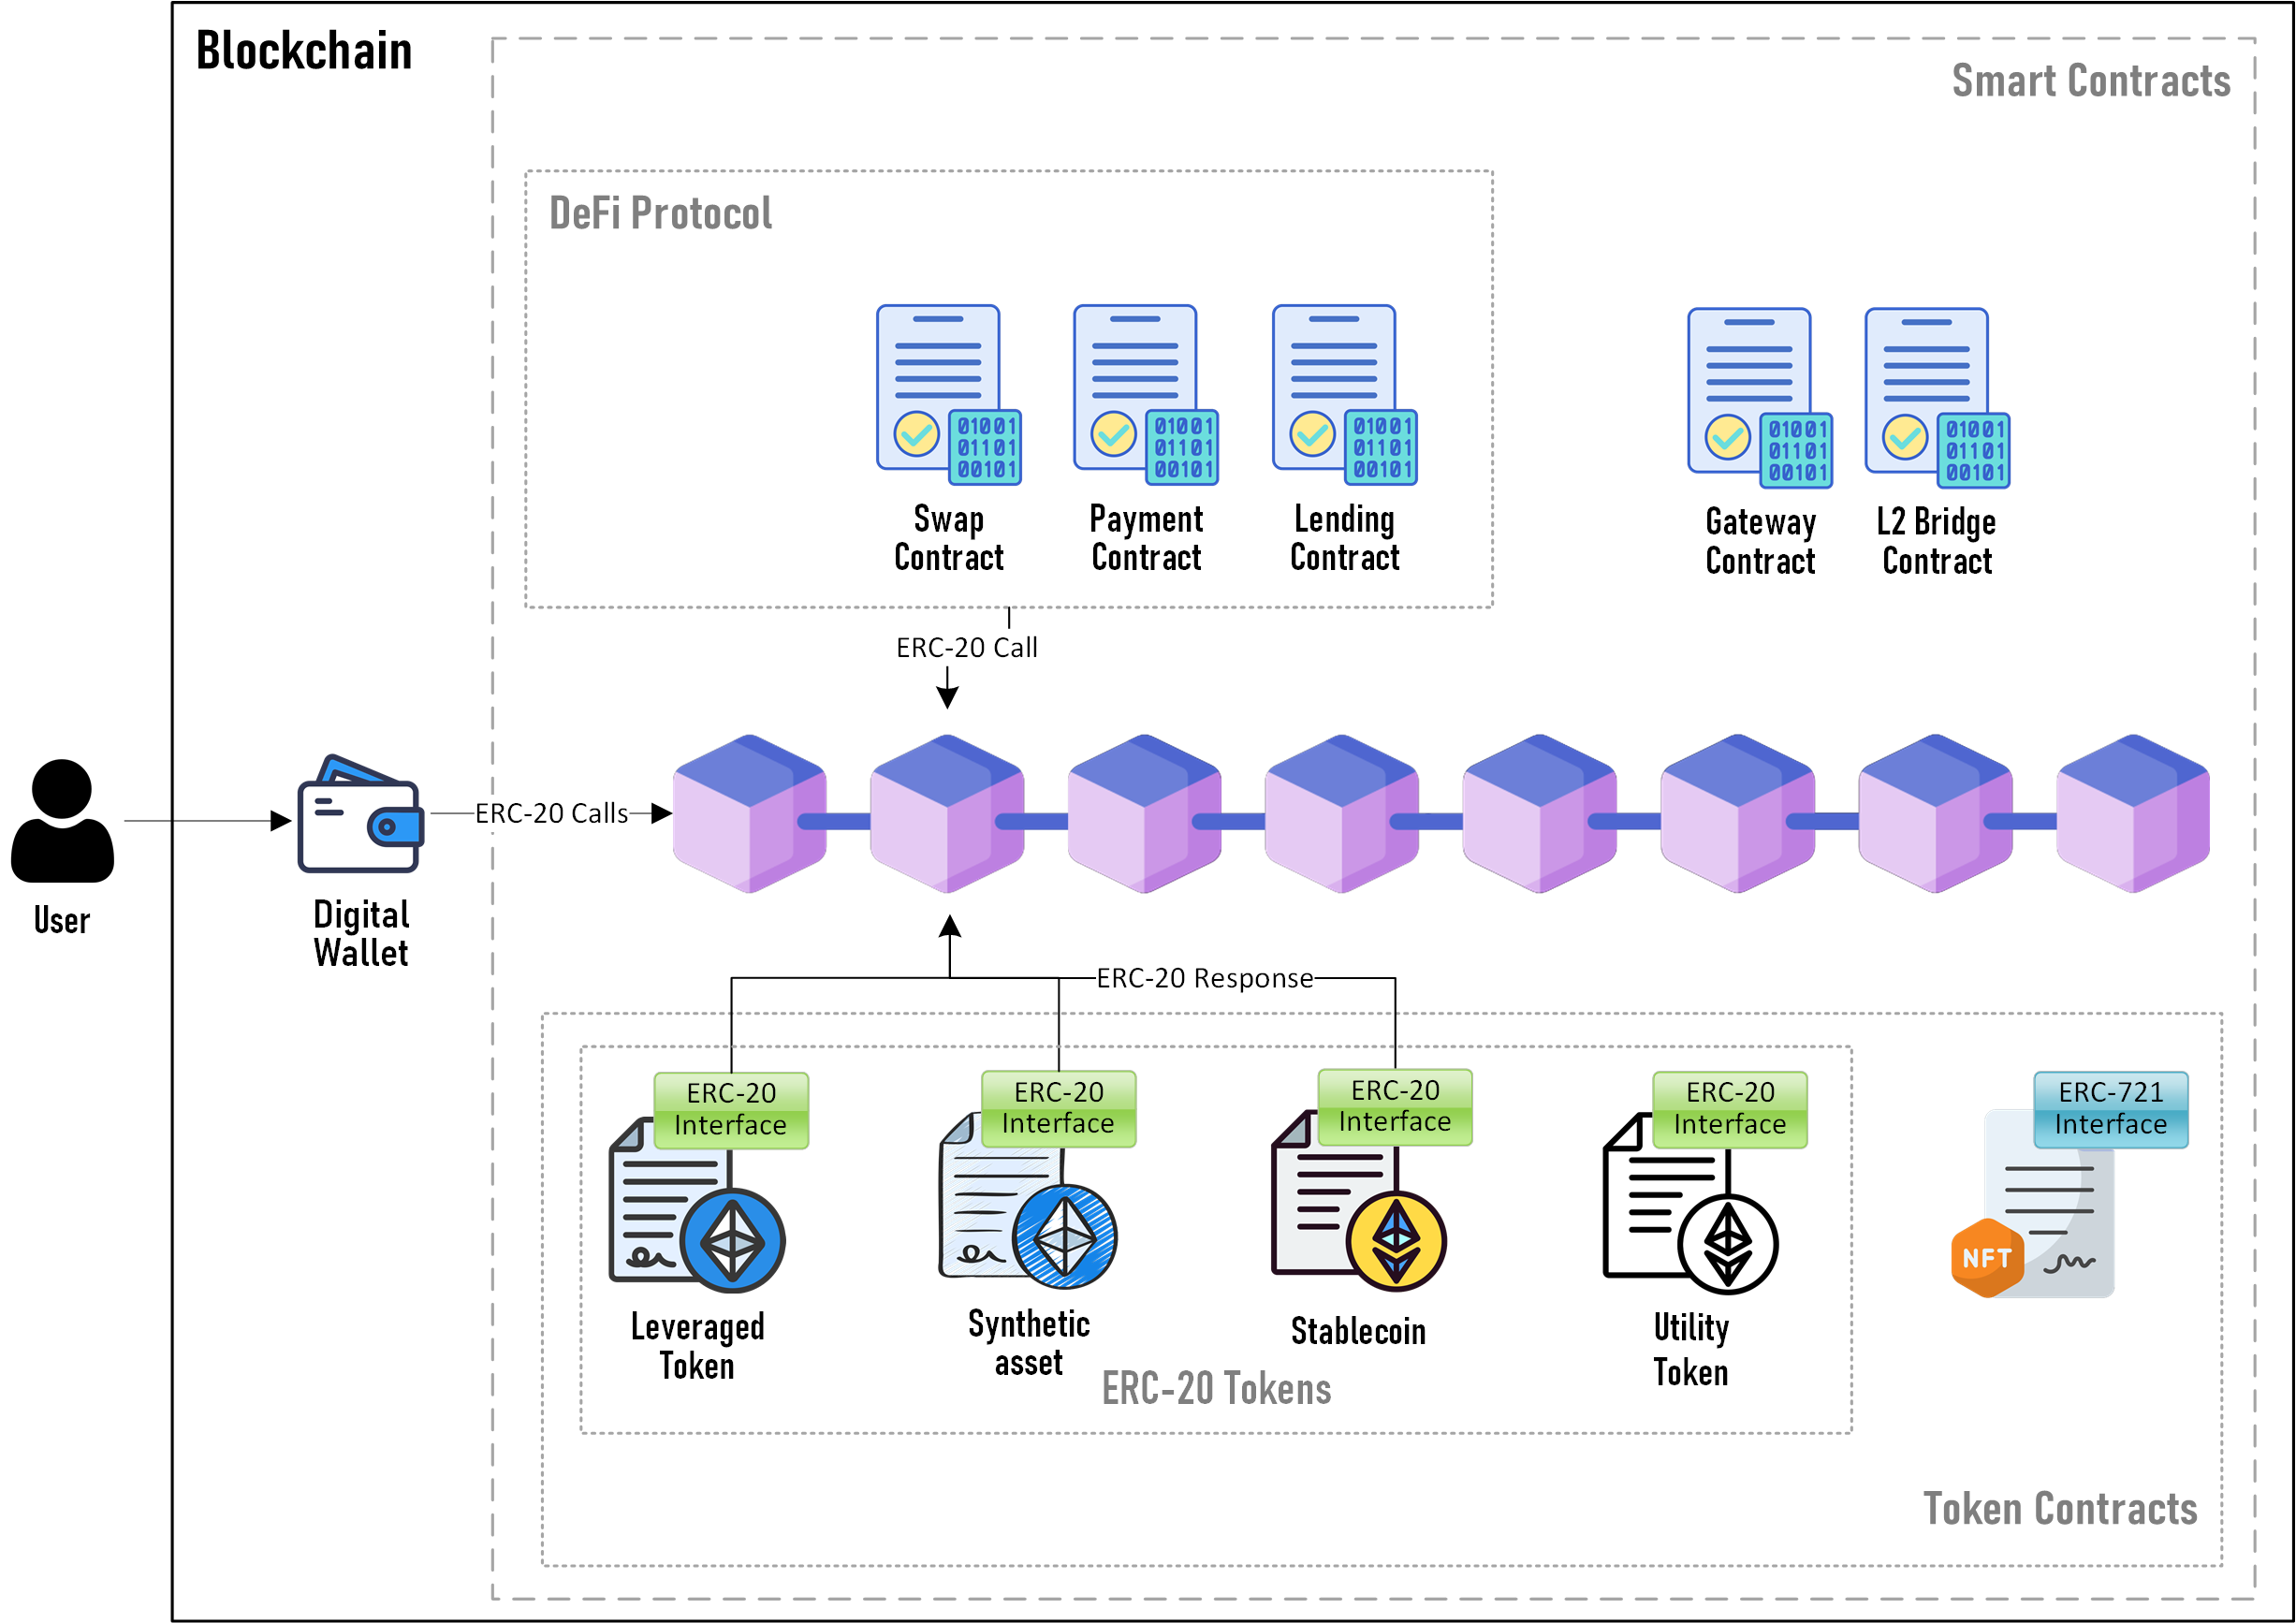
\includegraphics[width=\textwidth,keepaspectratio]{interaction.png}
	\caption[The Ethereum and DeFi ecosystem]{Place of ERC-20 tokens and LVTs within the Ethereum and DeFi ecosystem. At the core, there is the Ethereum Blockchain layer, which supports smart contracts. ERC-20 tokens are divided into categories such as leveraged tokens, stablecoins, and utility tokens, connecting to DeFi protocols like lending platforms and decentralized exchanges. Most interactions with fungible tokens follow the interface defined by the ERC-20 standard.}
	\label{fig:interaction}
\end{figure}

\subsection{ERC-20 Tokens: A Key Component of DeFi}
ERC-20 tokens contribute significantly to the functionality of the Ethereum blockchain and DeFi. While numerous core aspects of blockchain deserve study, ERC-20 tokens stand out for several reasons. They represent the fundamental building blocks of DeFi. Nearly all decentralized applications (dApps) rely on this token standard for asset tokenization, encompassing stablecoins, governance tokens, and utility tokens. As shown in gray in Figure \ref{fig:tokens}, majority of Ethereum-based tokens follow this standard. Moreover, ERC-20 tokens power key DeFi components such as liquidity pools, lending protocols, decentralized exchanges, and governance systems.

\begin{figure}[t]
	\centering
	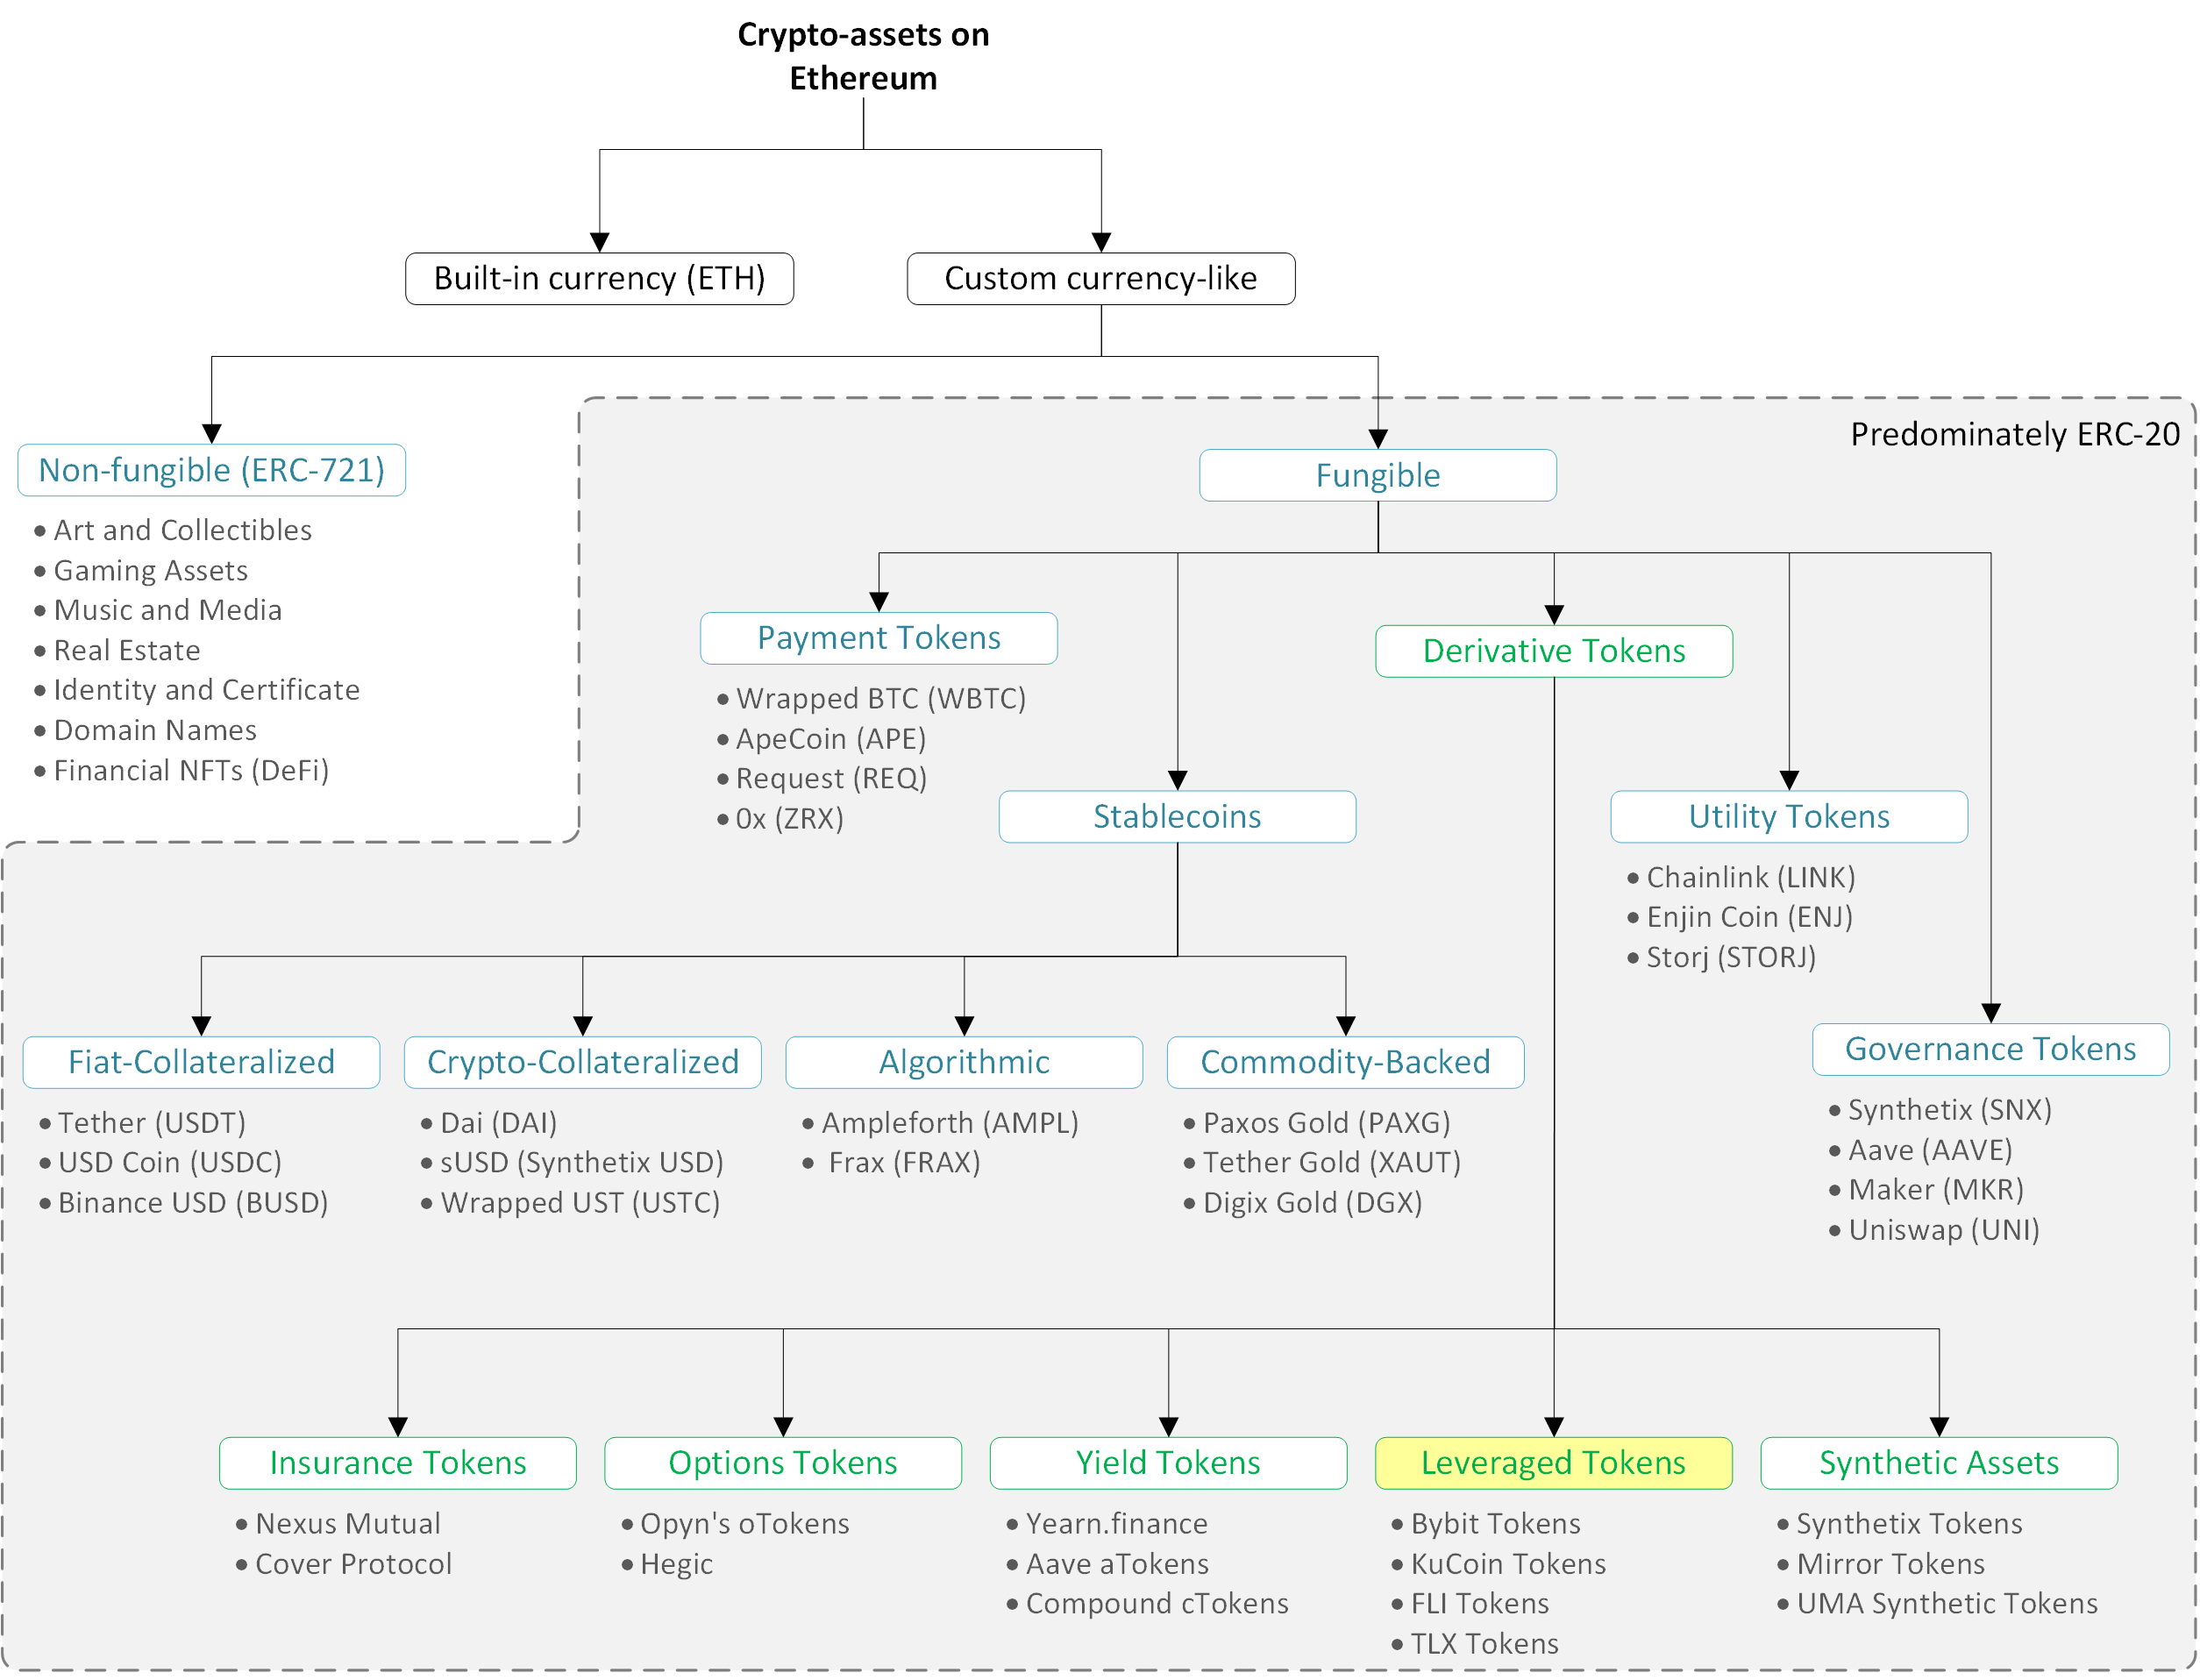
\includegraphics[width=\textwidth,keepaspectratio]{tokens.png}
	\caption[Categorization of the different types of tokens]{Categorization of the different types of tokens based on their functionality, standard protocols, and use cases within the Ethereum ecosystem. More than 98\% of fungible tokens follow ERC-20 standard.}
	\label{fig:tokens}
\end{figure}

ERC-20 tokens are technically smart contracts that follow a standardized interface, defining a set of rules and functions that each token must implement to ensure compatibility with other smart contracts and dApps. Like any programming code, they are prone to security vulnerabilities. By examining ERC-20 tokens, we gain insights into the core mechanics of decentralized asset representation and movement, which are required for enhancing security of these instruments. We explore the security challenges associated with ERC-20 tokens to identify potential enhancements and ensure compliance with best practices. This contribution strengthens the security of ERC-20 tokens, reinforcing their pivotal role in DeFi ecosystem.

\subsection{Leveraged Tokens: Complexity and Investor Safeguards}
Unlike ERC-20 tokens, leveraged tokens (LVTs) are not a critical infrastructure component of the blockchain. However, they present a layer of complexity that makes them worth exploring in academic research. Many users are attracted to LVTs due to their potential for amplified returns but often fail to fully grasp the technical details, particularly the risks associated with volatility decay, rebalancing mechanisms, or the impact of market movements in adverse directions. This lack of understanding may lead to common missteps, where users overestimate the gains of these tokens or underestimate their exposure to losses. By researching LVTs, we aim to shed light on these intricacies (see Table \ref{tab:risks}), helping both developers and users better comprehend the mechanisms at play and mitigating the associated risks.

\ExecuteMetaData[sections/tables]{tab-risks}

\section{Contributions and Outline} 
The structure of this dissertation follows an incremental research approach~\cite{Incremental_Research}, where the latest contributions are built on earlier findings, proposes solutions, and validates them through comparative analysis and integration. It is organized in the following chapters.

\subsection{Chapter \ref{ch:background}: Background} We provide an overview of key blockchain technologies, including the ERC-20 token standard, security auditing tools, and practices used to assess smart contract vulnerabilities. Additionally, we explore the concept of financial leverage and its application in crypto markets, such as lending platforms and futures markets. This chapter establishes the fundamental principles and protocols necessary for understanding the decentralized design, security considerations, and market dynamics discussed in subsequent chapters.

\subsection{Chapter \ref{ch:multiple}: Resolving the Multiple Withdrawal Attack on ERC20 Tokens}
We focus on Ethereum tokens, particularly ERC-20 tokens, which are integral to dApps deployed on Ethereum and other EVM-compatible chains. The ERC-20 standard is widely used and interoperable with numerous dApps, user interface platforms, and web applications. A key security issue, the \mwa, has existed since 2016 and involves the \texttt{approve} method, allowing malicious users to exploit token approvals. Understanding how the attack works aids in the process of mitigating it. Moreover, evaluating the proposed mitigations helps determine the extent to which they address the attack. If none are satisfactory, a new proposal will be required. In this regard, we answer RQ3 as the primary research question, followed by 5 guiding questions:

\noindent (RQ3) Are there any open security vulnerabilities in the ERC-20 protocol that remain unaddressed?
\begin{enumerate}[label={(RQ3.\arabic*)},leftmargin=*]
	\item How does the \mwa work, and why is its mitigation important?
	\item Where should this attack be prevented, and what does an ideal solution looks like?
	\item What efforts have been made to address this vulnerability, and to what extent have they been effective?
	\item Can the \mwa be mitigated while ensuring backward compatibility and adherence to the ERC-20 standard?
	\item How would a potential solution impact the token's performance or gas requirements?
\end{enumerate}
\paragraph{Contributions.} We evaluate 10 proposed mitigations for the \mwa and develop a set of criteria that encompass (i) backward compatibility, (ii) DeFi interoperability, (iii) adherence to the ERC-20 standard, and (iv) attack mitigation. Since no mitigation is fully satisfactory, we study in detail possible implementations of ERC-20's \texttt{approve} and \texttt{transferFrom} methods. We then develop two additional solutions: one deploys a secure \texttt{approve} method but does not adhere to the specifications of the ERC-20 standard. The second, mitigates the attack by securing the \texttt{transferFrom} method and fully satisfies the ERC-20 standard specifications. This solution requires 37\% more gas compared to the non-secure implementation, which we believe is justifiable to protect users investing in ERC-20 tokens.

\subsection{Chapter \ref{ch:tokenhook}: TokenHook: Secure ERC-20 Smart Contract}
Ethereum has undergone numerous security attacks, collectively causing more than US\$100M in financial losses~\cite{DAO1,PeckShield,PartiyMultiSig,MyEthWallet,ParityFirstHack,ParitySecondHack}. Drawing from the \mwa work~\cite{MultipleWithdrawal}, it seems reasonable to investigate all potential security vulnerabilities affecting ERC-20 tokens and systematize them. Additionally, assessing the effectiveness of popular static analysis tools designed for smart contracts can identify potential inconsistencies and false positives, highlighting areas for improvement. Although prior research has addressed smart contract vulnerabilities~\cite{EthSecServ}, there are still concerns on the security of ERC-20 tokens that can be answered by the primary research question RQ4 followed by 3 guiding questions:

\noindent (RQ4) How can known ERC-20 security risks be classified to improve overall token security?
\begin{enumerate}[label={(RQ4.\arabic*)},leftmargin=*]
	\item What are other known vulnerabilities in ERC-20 tokens, and how can they be systematically categorized to improve security practices?
	\item Can a new ERC-20 implementation, enhance security and software diversity compared to existing Solidity and Vyper implementations?
	\item How effective are widely-used auditing tools in detecting security vulnerabilities in ERC-20 token implementations, and can they replace the need for expert human security reviews?
\end{enumerate}
\paragraph{Contributions.} We study all known vulnerabilities and cross-check their relevance to ERC-20 token contracts, systematizing a comprehensive set of 82 distinct vulnerabilities and best practices. We then use our specialized domain knowledge to provide a new ERC-20 implementation, TokenHook, which is open source and freely available in both Vyper and Solidity. It aims to increase software diversity, as currently no Vyper ERC-20 implementation is considered a reference, and only one Solidity implementation is actively maintained. Compared to this implementation, TokenHook offers enhanced security properties and stronger compliance with best practices. Finally, we use TokenHook as a benchmark to assess the completeness and precision of seven widely used auditing tools for detecting security vulnerabilities. We conclude that while these tools offer some value, they cannot replace the expertise of a security professional in developing and reviewing smart contract code.

\subsection{Chapter \ref{ch:shortfall}: A Shortfall in Investor Expectations of Leveraged Tokens}
We examine leveraged tokens (LVTs) as emerging crypto-assets primarily issued by centralized exchanges. These tokens are modeled after the concept of leveraged ETFs (LETFs) in traditional markets, offering amplified gains and losses relative to the underlying asset. Since 2019, more than 1,600 leveraged tokens have been introduced. By analyzing key aspects such as underlying assets, blockchain interaction, types of leveraged products, and fund management algorithms, we can formalize LVT dynamics and mechanics of their constituent components. Analyzing these aspects clarifies how the tokens achieve leverage and maintain their structure over time. Additionally, it helps investors to understand the functionality of leveraged funds, rebalancing mechanisms, and potential risks. This is crucial for making informed investment decisions that we address through the primary research question RQ5 followed by 4 guiding questions:

\noindent (RQ5) What are Leveraged Tokens (LVT), and what limitations exist in their current operations?
\begin{enumerate}[label={(RQ5.\arabic*)},leftmargin=*]
	\item What information is accessible to LVT traders, and how transparent are these investment vehicles in terms of their structure and risk exposure?
	\item  Are LVTs adequately financially backed and able to effectively track their leverage ratios, ensuring they deliver the expected returns to investors?
	\item To what extent are LVTs tied to specific exchanges, and what risks, such as front-running, arise from this dependency?
	\item How do LVT fees and tracking errors compare to those of traditional LETFs, which are commonly used by investors as a baseline for comparison?
\end{enumerate}
\paragraph{Contributions.} We analyze more than 1,600 LVTs from 10 issuers, and show that 99.9\% of LVTs are centralized, which implies they are only accessible internally within the ecosystem of the exchange itself. 80\% of them do not interact with the blockchain, leading to the lack of transparency in transactions, holders, custody, and auditing. Moreover, 53\% of the issuers do not disclose the total supply, making challenging for investors to trade LVTs by their fair market price. The absence of uniform standards in LVT implementation has led to unpredictable technical and financial performance. 

Additionally, 41\% of LVTs may have been issued without sufficient financial support upon their launch where required future products were launched with delay. About 97\% of them are vulnerable to front-running during well-known events. LVTs have higher leverage deviation from the advertised ratio compared to LETFs because of inconsistencies in the management of funds or inefficiencies in rebalancing algorithms. Holding both LETFs and LVTs for extended periods of time impacts the performance, referred to as volatility decay. LVTs also normally have higher management fees than LETFs, which negatively affects the performance of the fund relative to the expected return. Our analysis provides valuable insights for crypto investors, developers, and auditors, offering a framework for understanding LVT mechanics, risks, and market impact.

\subsection{Chapter \ref{ch:leveredge}: LeverEdge: On-Chain Leveraged Tokens} 
The research literature~\cite{shortfall,khomyn2020value,szpruch2024leveraged,Sullivan_2009} has shown that LVTs in the crypto market diverge from the expected returns of LETFs, leading to notable deficiencies. Ten deficiencies are identified, largely due to the absence of a standardized implementation framework. This is a motivation for academia to explore solutions aimed at overcoming the limitations of LVTs. This is critical because users purchase LVTs under the assumption that these tokens will merely amplify the return of the underlying asset (ETH, BTC, \etc). However, they remain unaware of the internal mechanics of these tokens, such as daily rebalancing and the volatility decay, which can result in significant losses when the token is held for an extended period. Functional aspects of LVTs can be clarified by addressing the primary research question RQ6 followed by 4 guiding questions. It can assist users in better understanding LVTs before making investment decisions.

\noindent (RQ6) What solutions have been proposed to improve LVT functionality, and can a decentralized design eliminate existing shortcomings?
\begin{enumerate} [label={(RQ6.\arabic*)},leftmargin=*]
	\item What is the impact of current deficiencies on the performance of LVTs?
	\item What solutions have been proposed or implemented to address these issues, and how successful have they been?
	\item Can a new decentralized design like LeverEdge eliminate existing shortcomings, and how does its efficiency compare to current decentralized LVTs on Ethereum?
	\item Are there any inherent flaws in LeverEdge that need to be addressed in future work?
\end{enumerate}
\paragraph{Contributions.} We review six decentralized LVTs and evaluate the extent to which they address the identified deficiencies. Despite notable attempts, a closer examination of their functionality reveals ongoing shortcomings that still need to be resolved. In response, we propose a fully decentralized design model, LeverEdge, deployed on the Ethereum blockchain. Unlike existing centralized implementations, LeverEdge is entirely on-chain, addressing most of the identified deficiencies. However, this approach introduces challenges related to blockchain limitations, such as latency, scalability, and gas fees. To mitigate these, we developed a new L1-L2 hybrid model, which has passed security checks and can serve as a reference for future decentralized LVT deployments on EVM-compatible chains. 

LeverEdge has been evaluated under similar conditions as other LVTs, demonstrating its capability to address the recognized flaws. It employs perpetual futures to generate leveraged exposure and incorporates a cross-chain mechanism for compatibility with various L2 ecosystems. Designed with a focus on composability, it is deployed on Ethereum, and its open-source code has successfully passed security audits, making it a blueprint for developing new decentralized LVTs or transitioning existing centralized versions to decentralized solutions. The ultimate goal is to enhance investor protection by reducing risks associated with centralized control and improving the transparency of LVT operations.

\subsection{Chapter \ref{ch:remarks}: Concluding Remarks}
We summarize the key findings and contributions of our research in this chapter. It highlights the significance of the results, how they were achieved, and offering suggestions for potential directions in future work.

%In terms of scope, the dissertation focuses on two key areas within the DeFi ecosystem: (i) enhancing the security of ERC-20 tokens and, (ii) addressing shortcomings of LVTs. Security vulnerabilities in supplementary layers (\eg consensus, data, network) impact the entire Ethereum blockchain but do not necessarily ERC-20. Thus, vulnerabilities in these layers are considered beyond the scope. In the case of LVTs, there remains a risk of front-running by miners, who could deliberately include rebalancing transactions in future blocks and delay them to prioritize their own. In our design, miner-related front-running risks are excluded from the scope, but the risk posed by other traders has been thoroughly addressed.